\documentclass{sigchi}

% Use this command to override the default ACM copyright statement (e.g. for preprints). 
% Consult the conference website for the camera-ready copyright statement.


%% EXAMPLE BEGIN -- HOW TO OVERRIDE THE DEFAULT COPYRIGHT STRIP -- (July 22, 2013 - Paul Baumann)
\toappear{\scriptsize Permission to make digital or hard copies of all or part of this work for personal or classroom use is granted without fee provided that copies are not made or distributed for profit or commercial advantage and that copies bear this notice and the full citation on the first page. Copyrights for components of this work owned by others than the author(s) must be honored. Abstracting with credit is permitted. To copy otherwise, or republish, to post on servers or to redistribute to lists, requires prior specific permission and/or a fee. Request permissions from permissions@acm.org. \\
{\emph{CHI 2014}}, April 26--May 1, 2014, Toronto, Ontario, Canada. \\
Copyright is held by the owner/author(s). Publication rights licensed to ACM. \\
ACM 978-1-4503-2473-1/14/04..\$15.00.\\
http://dx.doi.org/10.1145/2556288.2557256 }
\clubpenalty=10000 
\widowpenalty = 10000

% Arabic page numbers for submission. 
% Remove this line to eliminate page numbers for the camera ready copy
\pagenumbering{arabic}


% Load basic packages
\usepackage{balance}  % to better equalize the last page
\usepackage{graphics} % for EPS, load graphicx instead
\usepackage{times}    % comment if you want LaTeX's default font
\usepackage{url}      % llt: nicely formatted URLs

\usepackage{enumitem}

% llt: Define a global style for URLs, rather that the default one
\makeatletter
\def\url@leostyle{%
  \@ifundefined{selectfont}{\def\UrlFont{\sf}}{\def\UrlFont{\small\bf\ttfamily}}}
\makeatother
\urlstyle{leo}


% To make various LaTeX processors do the right thing with page size.
\def\pprw{8.5in}
\def\pprh{11in}
\special{papersize=\pprw,\pprh}
\setlength{\paperwidth}{\pprw}
\setlength{\paperheight}{\pprh}
\setlength{\pdfpagewidth}{\pprw}
\setlength{\pdfpageheight}{\pprh}

% Make sure hyperref comes last of your loaded packages, 
% to give it a fighting chance of not being over-written, 
% since its job is to redefine many LaTeX commands.
\usepackage[pdftex]{hyperref}
\hypersetup{
pdftitle={Smart Subtitles for Language Learning},
pdfauthor={LaTeX},
pdfkeywords={subtitles, language learning, interactive videos},
bookmarksnumbered,
pdfstartview={FitH},
colorlinks,
citecolor=black,
filecolor=black,
linkcolor=black,
urlcolor=black,
breaklinks=true,
}

% create a shortcut to typeset table headings
\newcommand\tabhead[1]{\small\textbf{#1}}

\usepackage{CJKutf8}

\usepackage{float}

\usepackage{stfloats}

% End of preamble. Here it comes the document.
\begin{document}

\title{Smart Subtitles for Vocabulary Learning}

\numberofauthors{2}
\author{
  \alignauthor Geza Kovacs \\
    \affaddr{Stanford University}\\
    \affaddr{Stanford, CA, USA}\\
    \email{gkovacs@stanford.edu}
  \alignauthor Robert C. Miller \\
    \affaddr{MIT CSAIL}\\
    \affaddr{Cambridge, MA, USA}\\
    \email{rcm@mit.edu} 
}

\maketitle

\begin{abstract}
Language learners often use subtitled videos to help
them learn. However, standard subtitles
are geared more towards comprehension than vocabulary learning,
as translations are nonliteral and are provided only for phrases, not vocabulary.
This paper presents Smart Subtitles, which are interactive subtitles
tailored towards vocabulary learning.
Smart Subtitles can be automatically generated from common video sources
such as subtitled DVDs.
They provide features such as vocabulary definitions on hover, and
dialog-based video navigation. In our pilot study
with intermediate learners studying Chinese,
participants correctly defined over twice as many new words
in a post-viewing vocabulary test when they used Smart Subtitles, compared to dual
Chinese-English subtitles.
Learners spent the same amount of time watching clips
with each tool, and enjoyed viewing videos
with Smart Subtitles as much as with dual subtitles.
Learners understood videos equally well using either tool,
as indicated by self-assessments
and independent evaluations of their summaries.
\end{abstract}

\keywords{
	subtitles; interactive videos; language learning
}

\category{H.5.2.}{Information Interfaces and Presentation}{Graphical User Interfaces}

\begin{figure}[!h]
\centering
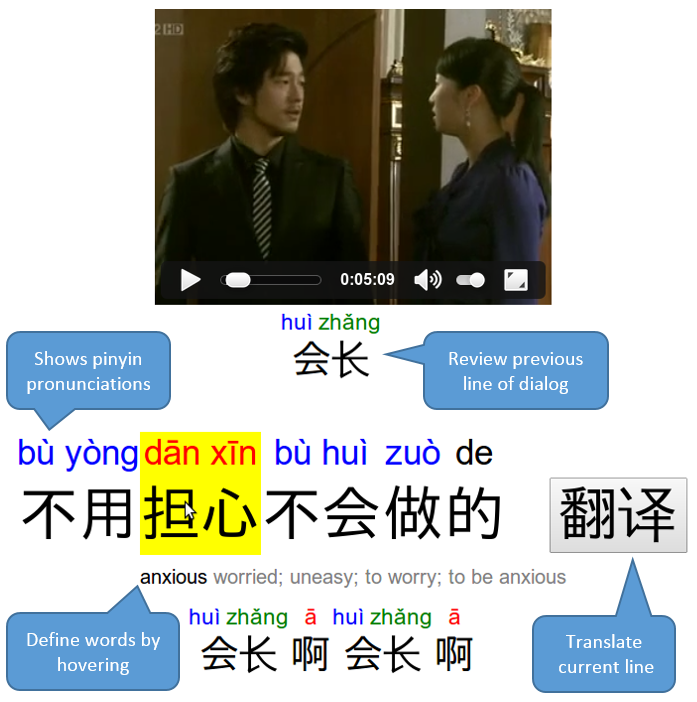
\includegraphics[width=\columnwidth]{smartsubs-features}
\caption{Screenshot of the Smart Subtitles system,
with callouts pointing out features that help users
learn vocabulary and navigate the video.}
\label{fig:figure1}
\end{figure}

\section{Introduction}

Students studying foreign languages often wish to enjoy authentic foreign-language video content. For example, many students cite a desire to be able to watch anime in its original form as their motivation for starting to study Japanese \cite{anime}. However, standard presentations of videos do not
provide good support for language learners. For example, if a learner were watching anime, and did not recognize a word in the dialog, the learner would normally have
to listen carefully to the word, pause the video, and look the word up in a dictionary. This is a time-consuming process which detracts from the enjoyability of watching the content. Alternatively, learners could simply watch a version that is dubbed, or a version with subtitles in their native language to enjoy the content. However, they might not learn the foreign language effectively this way.

There are other ways to show language learners videos to help them learn,
such as dual subtitles,
%Language educators have studied other ways to present videos to language learners.
%learners, such as reverse subtitles, dual subtitles, and GliFlix.
%Dual subtitles,
which simultaneously display subtitles in both the viewer's native
language and the language of the video.
%This is considered one of most effective
%ways to learn vocabulary from videos.
However, we believe we can do even better at teaching vocabulary
than dual subtitles
by introducing interactive features into the video player
to support common language learning tasks.

This paper presents \emph{Smart Subtitles}, an interactive, web-based
foreign-language video viewing tool
that aims to maximize vocabulary learning while ensuring that the learner
fully understands the video and enjoys watching it.

Smart Subtitles includes features to help
learners learn vocabulary and navigate videos.
It prominently displays a transcript of the foreign-language dialog, to
focus learners' attention on the foreign language.
Learners can view definitions for words in the video by hovering over them.
Learners can review the current and previous lines of dialog by clicking on them to replay the video.
If word-level translations are not enough for learners to understand the
current line of dialog, they can click a button to show a full translation.

Smart Subtitles can be automatically generated from a number
of video sources, such as DVDs. It also includes a novel algorithm for
extracting subtitles from hard-subtitled videos, where the subtitle is
part of the video stream. The Smart Subtitles system currently supports videos in Chinese,
Japanese, French, German, and Spanish, and can be extended to other languages
for which bilingual dictionaries are available.

We ran a within-subjects user study with 8 intermediate Chinese learners to compare Smart Subtitles against dual subtitles in their effectiveness in teaching vocabulary. After viewing a 5-minute video with one of the tools, participants took a vocabulary quiz,
wrote a summary of the video clip,
and filled out a questionnaire. They then repeated this procedure on another clip, with the other tool.

We found that learners correctly defined over twice as many new vocabulary
words when they viewed clips using Smart Subtitles, compared to dual subtitles.
However, as the vocabulary quiz was administered immediately after
viewing, this only tested short-term vocabulary retention.
The amount of time learners spent viewing the videos was the same in both conditions.
Users enjoyed
using Smart Subtitles to view videos, and rated it
significantly easier to learn vocabulary with the Smart Subtitles interface.
Their comprehension of the videos was equally high in both conditions,
as indicated by both self-assessments as well as expert ratings
of the quality of their video summaries.
Users used the vocabulary-hover feature extensively,
and viewed dialog-level translations for only a third of the lines,
suggesting that word-level translations
are often sufficient for intermediate-level learners to comprehend the video.
%, using it on
%75\% of lines of dialog. Users viewed dialog-level translations for only
%28\% of the lines of dialog, suggesting that word-level translations
%are often sufficient for intermediate-level learners to comprehend the video.

The main contributions of this paper are:

\begin{itemize}[noitemsep]
\item An interactive video viewer with features to help language learners
learn vocabulary and navigate videos.
\item A system for extracting subtitles from various sources, including
hard-subtitled video where the subtitles are baked into the video stream.
\item A system to automatically annotate subtitles with word definitions
and romanizations to display to language learners.
\item A pilot study that suggests that Smart Subtitles improves intermediate-level learners' short-term vocabulary learning relative to dual subtitles, with no changes in viewing times, enjoyment, or comprehension.
\end{itemize}

%The Smart Subtitles system 
%However, these presentation formats are unsatisfactory, because


% elaborate on contributions here!

\section{Related Work}

Video has several advantages as a medium for language learning.
By presenting vocabulary in the context of a natural dialog, as opposed to isolated drills,
video promotes \emph{contextualized learning}, helping learners understand how
vocabulary is actually used in the language \cite{videocontext}.
In classroom contexts, students are sometimes given supplemental materials
explaining vocabulary and concepts that appear in the video,
referred to as \emph{advance organizers}, which help combine the benefits of
drill-based learning with the context provided by videos \cite{advanceorganizer}.

Videos in foreign languages have been adapted for foreign viewers and languages learners in many ways. These are summarized in Figure~\ref{fig:figure2} and are described in more detail below.

\begin{figure}[!h]
\centering
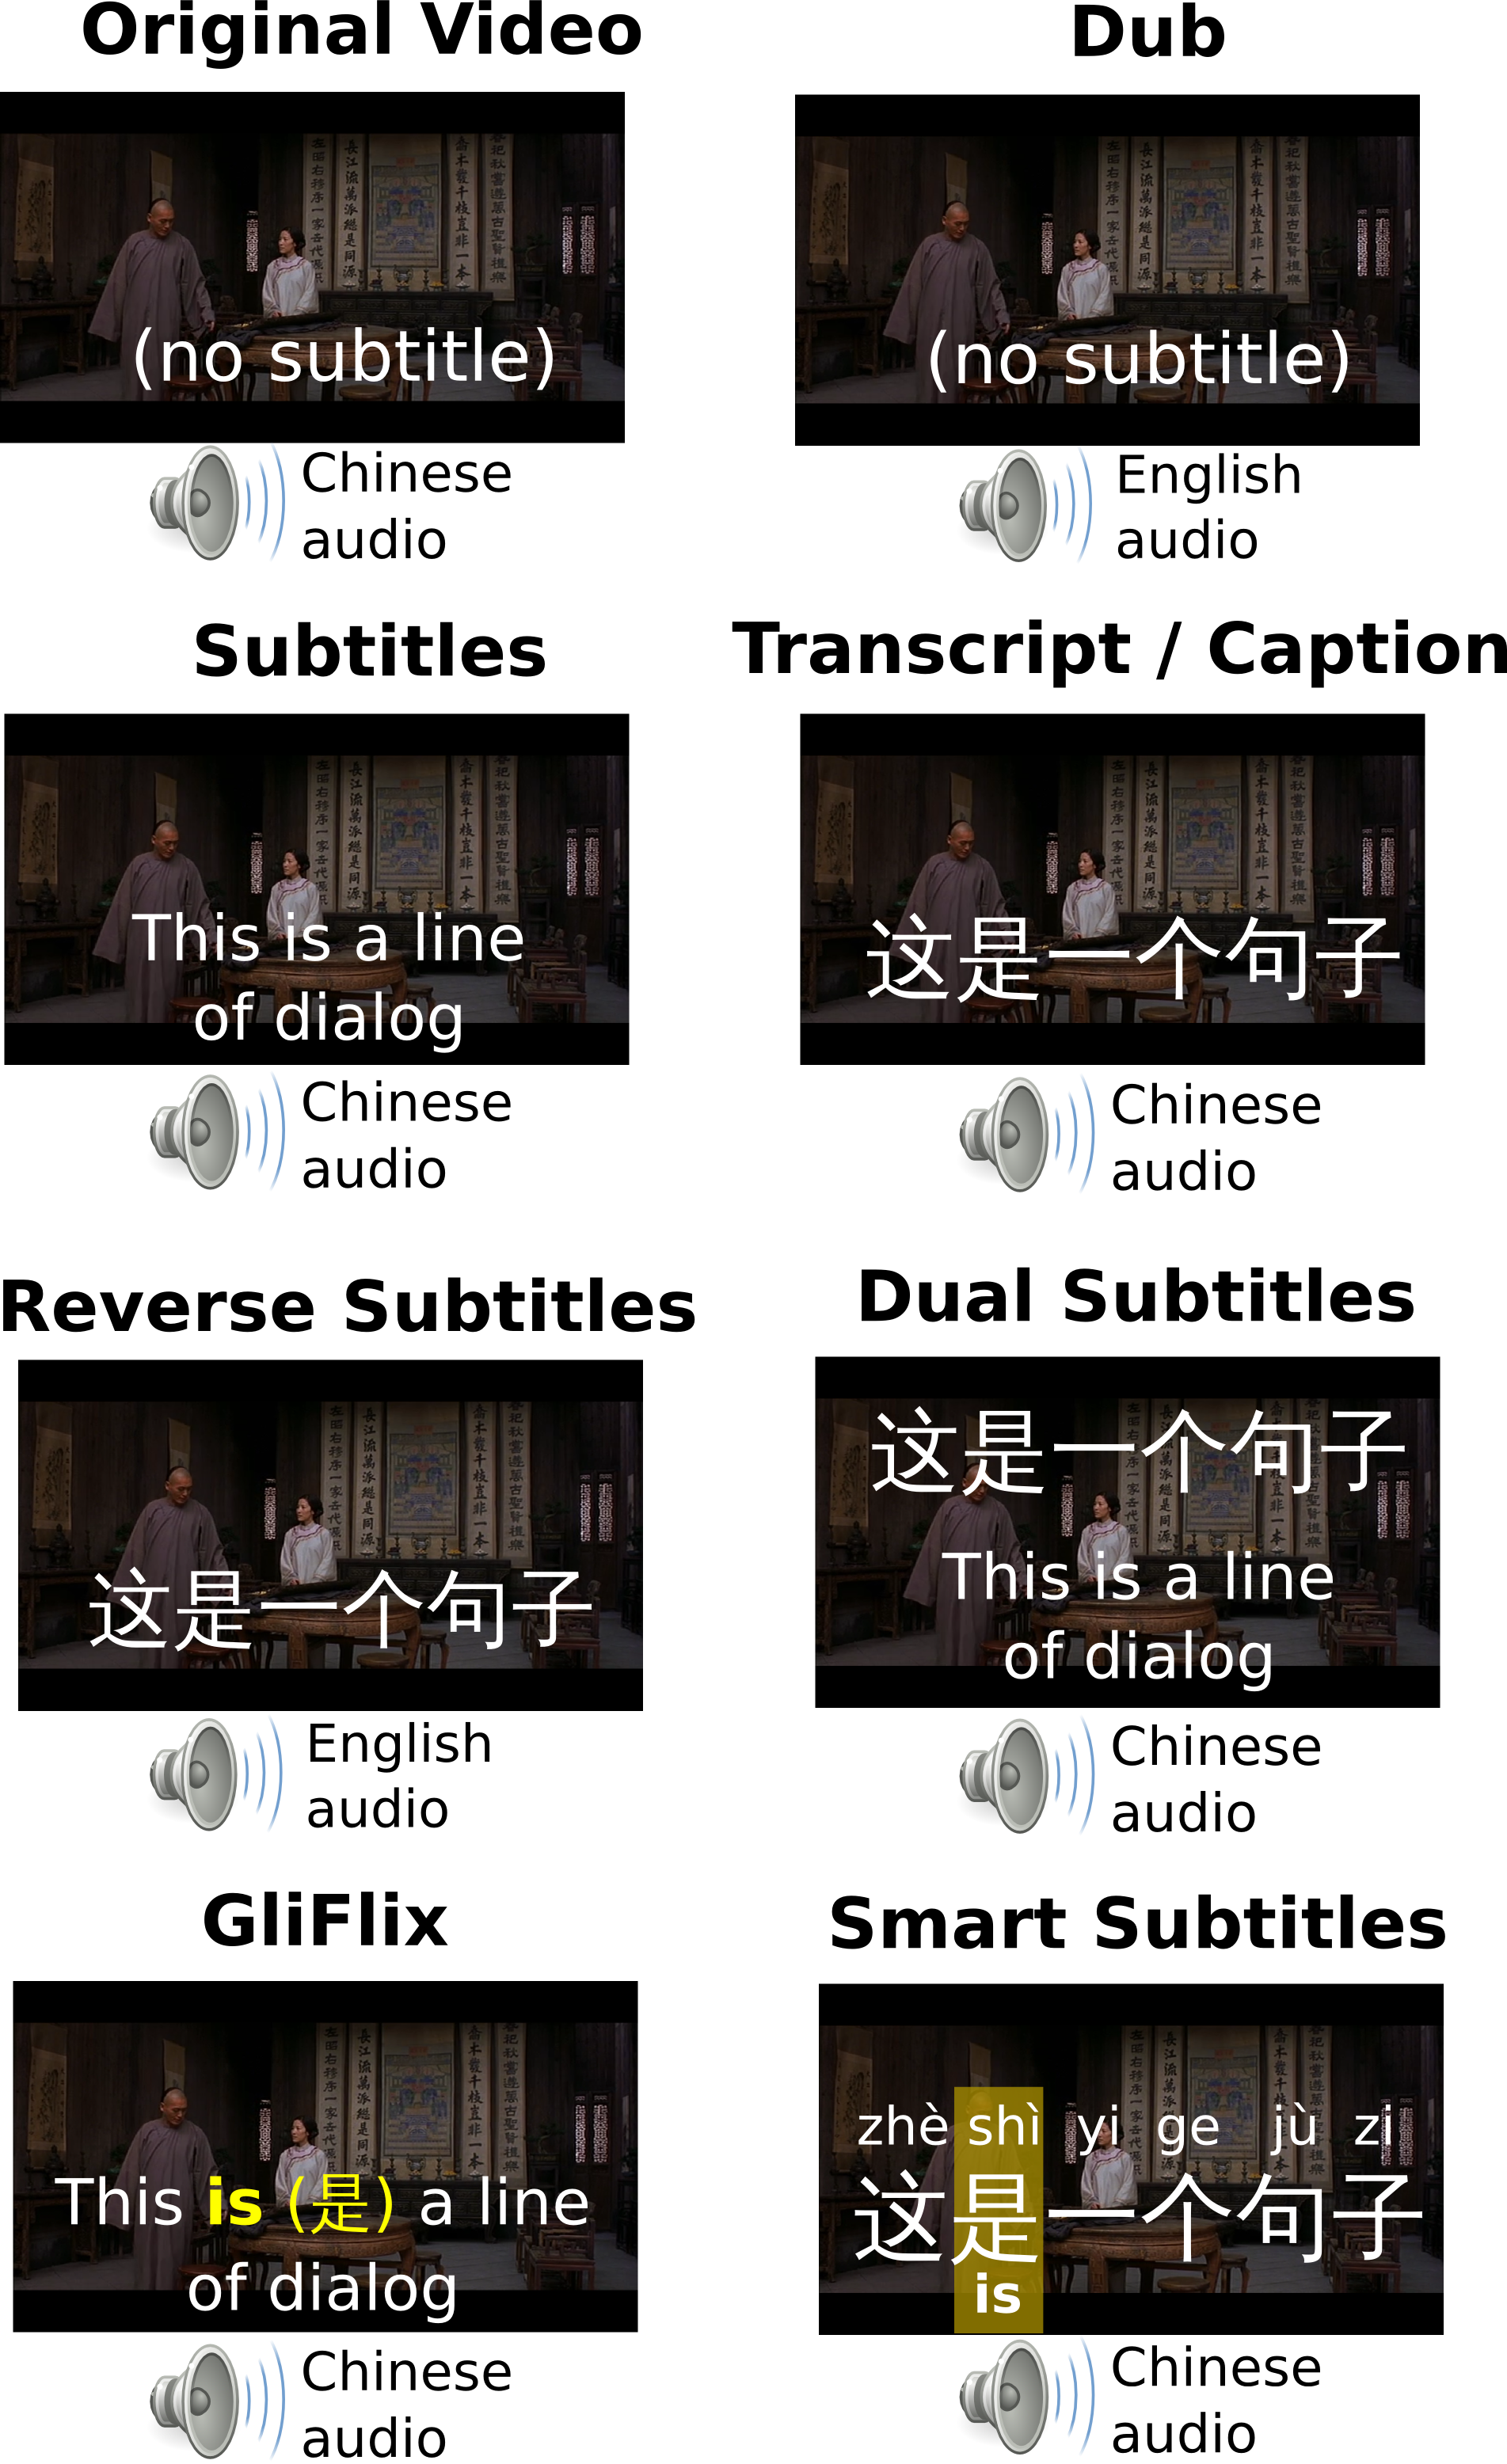
\includegraphics[width=\columnwidth]{subtitle-types-2column}
\caption{Mockups showing how Smart Subtitles
compares to existing ways that a Chinese video can be presented
to English-speaking viewers and language learners.
Note that GliFlix does not actually support Chinese.
To conserve space, this mockup only shows the vocabulary-learning features of Smart Subtitles, not the navigation features.}
\label{fig:figure2}
\end{figure}

\subsection{Presenting Videos to Foreign Viewers}

One approach used to adapt videos for viewers who do not understand the original language is \emph{dubbing}. Here, the original foreign-language voice track is replaced with a voice track in the viewer's native language.
Because the foreign language is no longer present in the dubbed version, dubbed videos are ineffective for foreign language learning \cite{dubbing}.

Another approach is to provide \emph{subtitles} with the video. Here, the foreign-language audio is retained as-is, and the native-language translation is provided in textual format, generally as a line presented at the bottom of the screen.
Thus, the learner will hear the foreign language, but will not see its written form.
%Therefore, they must pay close attention to the audio
%to learn the foreign language.

Subtitles have been extensively studied in the context of language learning,
with mixed results.
Some studies have found them to be beneficial for vocabulary acquisition, compared to watching videos without them \cite{danan2004captioning}.
That said, other studies have found them to provide little benefit to language learners in learning vocabulary \cite{danan1992reversed}. Additionally, the presence of subtitles are considered to detract attention from the foreign-language audio and pronunciation \cite{mitterer2009foreign}.
These mixed results on the effects of subtitles on language learning suggest that their effectiveness depends on factors such as learners' experience levels \cite{bianchi2008captions}.

\subsection{Presenting Videos to Language Learners}

%Whether or not videos should at all be presented to language learners with subtitles or similar aids is itself a matter of debate. Subtitles, in particular, are frowned upon, because they do nothing to deter learners from simply reading in their native language. Some language educators are of the opinion that since students will not have subtitles or similar aids when they visit the foreign country, then they should not be provided with any when viewing videos either. Nevertheless, various video comprehension aids have been experimented with in the context of language learning:

In addition to subtitles, there exist other techniques to aid language learning
while watching videos, described below.

\begin{figure*}[bp]
\centering
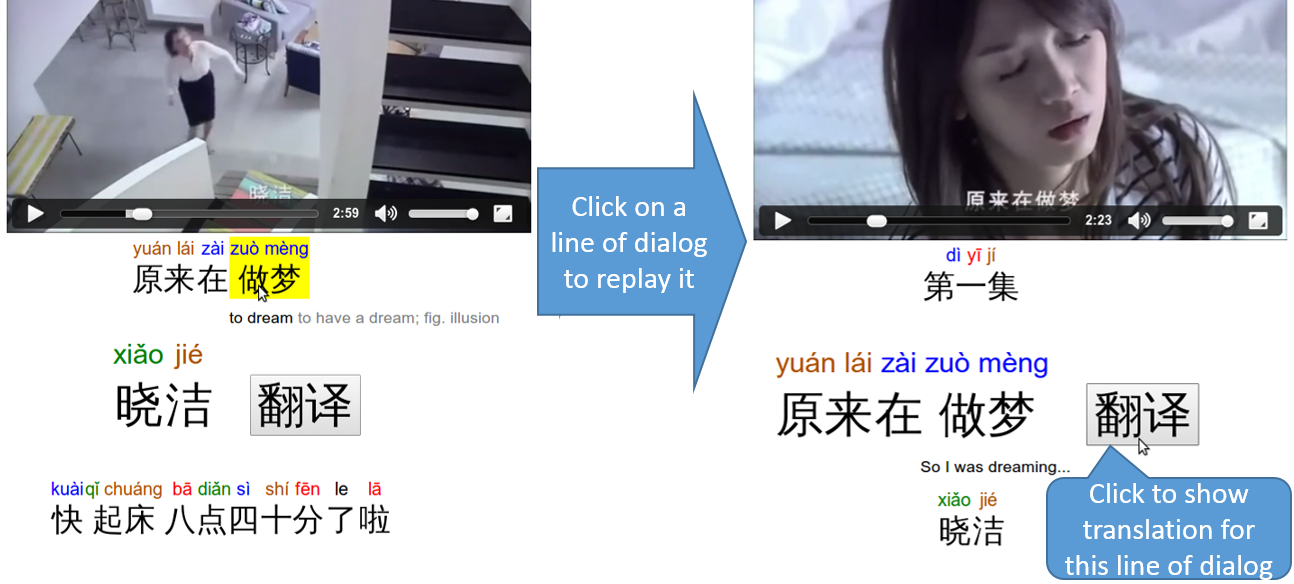
\includegraphics[width=2\columnwidth]{seekdialog-horizontal-translate-cropped2}
\caption{Smart Subtitles has several interactive features. It allows users to easily navigate the video and
review lines of dialog, either by clicking onto the line of dialog to replay,
scrolling the mouse wheel,
or pressing arrow keys on the keyboard. Users can hover over words
in the dialog to show their definitions, as shown on the left.
If word-level translations are not sufficient for users to understand the dialog, they can also press a button to show a translation for the current
line of dialog, as shown on the right.}
\label{fig:figure25}
\end{figure*}

With a \emph{transcript}, also known as a \emph{caption}, the video is shown along with the text in the
language of the audio, which in this case is the foreign language. Transcripts are generally used to
assist hearing-impaired viewers. However, they can also be beneficial to language learners for
comprehension, particularly if they have better reading ability than
listening comprehension ability \cite{danan2004captioning}. However,
for learners with only basic reading abilities,
using only a transcript can lead to decreased comprehension compared to subtitles \cite{bianchi2008captions}.



With \emph{reverse subtitles} \cite{danan1992reversed}, the video has an audio track and a single subtitle, just as with regular
subtitles. However, in reverse subtitles, the audio is in the native language, and
the subtitle shows the foreign language. This takes advantage of the fact that subtitle reading is
a semi-automatic behavior \cite{d2002foreign}, meaning that the presence of text on the screen tends to attract
people's eyes to it, causing them to read it. Therefore, this should attract attention to the foreign-language text. The presentation of the foreign language in written form may also be helpful to learners whose reading comprehension ability is higher than their listening comprehension ability. That said, because the foreign language is presented only in written form, the
learner may not end up learning pronunciations, especially with languages using non-phonetic writing systems such as Chinese.

With \emph{dual subtitles}, the audio track for the video is kept as the original, foreign language.
Dual subtitles simultaneously display a subtitle in the viewer's native language, and a transcript in the original language. This way, a learner can both read and hear the dialog in the foreign language, and still have a translation
available. Thus, of these options, dual subtitles provide the most information to the learner.
Dual subtitles have been found to be at least as effective for vocabulary acquisition as
either subtitles or captions alone \cite{raine2012incidental}.
However, in our own interviews with Chinese language learners who regularly viewed Chinese movies
with dual subtitles, they stated they generally read the English subtitles first to comprehend the video and often did not have time to read the Chinese subtitles.
This suggests that dual subtitles may not be sufficiently
directing the user's attention
towards the foreign language.

\emph{GliFlix} \cite{gliflix} is a variant on conventional native-language subtitles which adds translations to the foreign language for the most common words that
appear in the dialog. For example, for a French dialog, instead of ``This is a line of dialog", GliFlix would show ``This is (\emph{est}) a line of dialog", showing that \emph{is} in French is \emph{est}. In user studies with learners beginning to study French, they attain larger rates of vocabulary acquisition compared to regular
subtitles, but not dual subtitles. Compared to dual subtitles, GliFlix has the disadvantage that it shows only the most common vocabulary words in a dialog, so learners may not learn all the vocabulary in the video. Additionally, because GliFlix presents the foreign vocabulary in the order of the viewer's native language, it is likely less beneficial than dual subtitles for
other language-learning tasks such as learning pronunciation and grammar.

\section{Smart Subtitles Interface}

We developed a video viewing tool, Smart Subtitles, which provides
language learners with interactive features to help them learn vocabulary.
Smart Subtitles supports features for learning vocabulary and navigating dialogs, which are shown in Figure~\ref{fig:figure25} and will be discussed in this section. Smart Subtitles can be used by English speakers to view videos in Chinese, Japanese, French, German, and Spanish. %Smart Subtitles can be automatically generated for any video, provided that a caption is available.

Smart Subtitles is an interactive web application that runs in the user's browser. The user simply provides it with a video and a caption, from either a streaming service or from the local filesystem,
and the interactive video player will start once it finishes automatically
generating annotations.

\subsection{Exploratory Interviews}

We designed our interface based on informal interviews with 6 students enrolled in foreign language classes who self-reported that they often watched subtitled videos outside class.
We asked them what aids they used while watching videos, what they did when they encountered new words, and what potential features they might find useful for learning.

Interviewees reported that they rarely looked
up words when watching videos, but thought they would do so more if it were easier to do. Many also indicated that they wanted easier ways to review parts of the video dialog that they didn't understand. Our features for vocabulary learning and navigation were designed to address these needs.

\subsection{Vocabulary Learning Features}

To reduce the effort required for vocabulary lookups, our interface allows the user to hover over words in
the dialog to show their definitions, as shown in Figure~\ref{fig:figure25}.

Sometimes, word-level translations are not enough for the learner to comprehend the current line of dialog. To address these cases, Smart Subtitles includes a button that shows learners a translation for the currently displayed line of dialog when pressed, as shown in Figure~\ref{fig:figure25}.

Because poor ability to
read Chinese characters can limit the usefulness of Chinese and Japanese captions,
the interface shows learners how to pronounce
Chinese characters. For Chinese, it shows \emph{pinyin}, the standard romanization system for Chinese. For Japanese, it shows \emph{hiragana}, the Japanese phonetic writing system. These  writing systems are taught to learners in first-semester Chinese and Japanese classes.

Tones are an essential part of Chinese pronunciation that learners often struggle to remember. To make them more visually salient, Smart Subtitles color-codes the pinyin displayed according to tone, in addition to displaying the tone mark. The tone colorization scheme is taken from the \emph{Chinese through Tone and Color} series \cite{tonecolor}, which has been adopted by popular online dictionaries for Chinese learners \cite{mdbg}.

\subsection{Navigation Features}

To address interviewees'
desire for easy ways to review unfamiliar lines of dialogs, in our interface, clicking on a section of the dialog will
seek the video to the start of that dialog.

Additionally, because prior work suggests that learners are able to comprehend videos better when
they are able to navigate videos according to syntactically meaningful chunks of dialog \cite{shea2000leveling}, we enable easy seeking through the video based on dialog. The transcript is prominently shown, and can be navigated by pressing the up/down keys, scrolling, or clicking on lines of dialog, as shown in Figure~\ref{fig:figure25}. Users can also search the video for occurrences of particular words in the dialog.

\section{Implementation}

Smart Subtitles faces several implementation challenges, such as extracting subtitles from various video, listing vocabulary words, and determining their definitions and romanizations. This section will discuss techniques for addressing these challenges.

Smart Subtitles are automatically generated from 
captions with the assistance of dictionaries and 
machine translation. Our implentation currently supports Chinese, Japanese, French, German, and Spanish, but support for other languages can easily be added if a bilingual dictionary is available.

The Smart Subtitles system
is implemented as 2 main parts:
a system that extract subtitles and captions from videos,
and a web application that learners use to play interactive videos.

\subsection{Extracting Subtitles from Videos}

Our system takes digital text captions in either the SubRip \cite{subrip} or Web Video Text Tracks (WebVTT) formats \cite{webvtt} as input.
These are plain-text formats that specify the textual lines of dialog, along with their respective display times.
Users can download these from
various online services, such as Universal Subtitles.
However, many possible sources of subtitles either
do not come with timing information, or are in
non-textual formats, so we have developed 
a subtitle extraction system so that Smart Subtitles
can be used with a broader range of videos.
An overview of the subtitle extraction process
is shown in Figure~\ref{fig:figure3}.

\begin{figure}[!h]
\centering
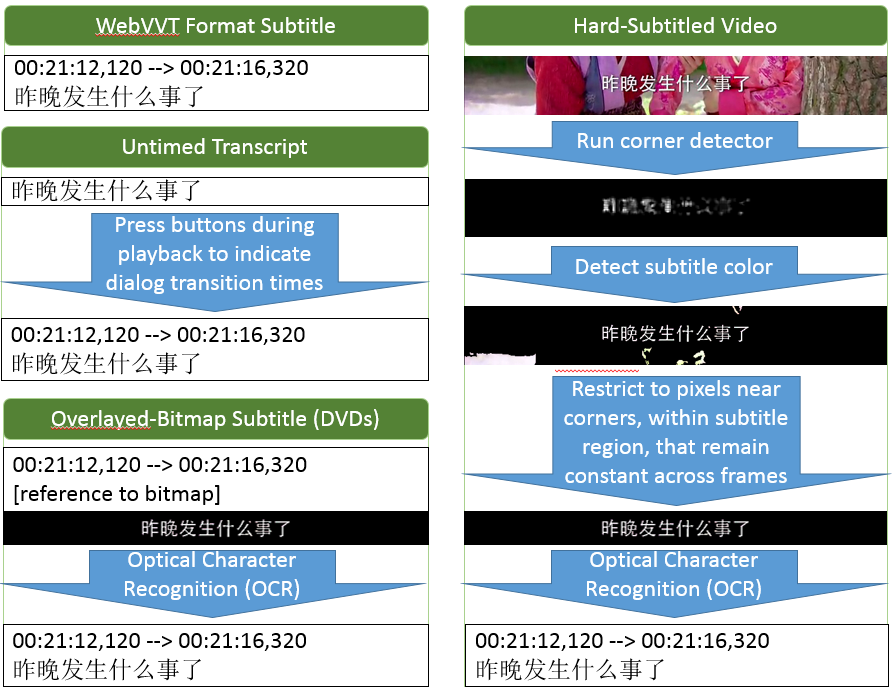
\includegraphics[width=\columnwidth]{subtitle-sources}
\caption{An overview of the sources that the Smart Subtitles system can extract subtitles from, and what the process of subtitle extraction consists of for each source.}
\label{fig:figure3}
\end{figure}

\subsubsection{Extracting Subtitles from Untimed Transcripts}

For many videos, a transcript is available, but the timing information
stating when each line of dialog was said is unavailable.
Examples include transcripts of lectures on sites such as
OpenCourseWare and lyrics for music videos.

It is possible to add timing information to videos automatically based on speech recognition techniques, which is called \emph{forced alignment} \cite{sailalign}.
However, we found that existing software for doing forced alignment
yields poor results on certain videos, particularly those with background
noise.

Thus, to generate timing information,
we wrote a timing annotation interface where an annotator
views the video, and presses the down arrow key whenever a new
line of dialog starts.
We gather this data for several annotators to guard against errors,
and use it to compute the timing information for the transcript,
generating a WebVTT-format subtitle that we can then provide to the Smart Subtitles system.

\subsubsection{Extracting Subtitles from Overlayed-Bitmap Formats}

Overlayed-bitmap subtitles are pre-rendered versions of the text which are overlayed onto the video when playing. They consist of an index mapping time-ranges to the bitmap image which should be overlayed on top of the video at that time. This is the standard subtitle format used in DVDs, where it is called VobSub.

Because we cannot read text directly from the overlayed-bitmap images in DVDs, Smart Subtitles uses Optical Character Recognition (OCR) to extract the text out of each image. Then, it merges this with information about time ranges to convert them to the WebVTT subtitle format. Our implementation can use either the Microsoft OneNote \cite{onenote} OCR engine, or the free Tesseract \cite{tesseract} OCR engine.

\subsubsection{Extracting Subtitles from Hard-Subtitled Videos}

Many videos come with \emph{hard subtitles}, where the subtitle is baked into the video stream. Hard subtitles have the advantage that they can be displayed on any video player. However, hard subtitles have the disadvantage that they are non-removable. Additionally, hard subtitles are difficult to extract machine-readable text from, because the pixels representing the subtitle must first be isolated from the rest of the video, before we can apply OCR to obtain the text. Existing tools that perform this task, such as SubRip, are time-consuming, as they require the user to specify the color and location of each subtitle line in the video \cite{subrip}.

That said, hard-subtitled videos are ubiquitous, particularly online. Chinese-language dramas on popular video-streaming sites such as Youku are frequently hard-subtitled in Chinese. Thus, to allow Smart Subtitles to be used with hard-subtitled videos, we devised an algorithm which can identify and extract Chinese subtitles from hard-subtitled videos.

The hard-subtitle extraction problem is conceptually similar to the
background removal problem in machine vision, which aims to isolate foreground objects from background images \cite{backgroundsubtraction}.
However, our hard-subtitle extraction algorithm differs from background-removal algorithms in that it explicitly takes advantage of a number of properties of subtitles, listed below:

\begin{itemize}[noitemsep]
\item Subtitles in the same video are of the same color, with some variance due to compression artifacts.
\item Subtitles in the same video are consistently shown in the same vertical region of the screen.
\item The position of subtitles is static, so they do not move around and are not animated.
\item Characters in the subtitle have many corners. This is a Chinese-specific assumption, owing to the graphical complexity of Chinese characters.
\end{itemize}

Our hard-subtitle extraction algorithm first attempts to determine the color
of the subtitle. To do so, it first runs the Harris corner detector \cite{harris1988combined}
on each frame of the video. Then, it computes a histogram of color values of pixels near corners, buckets similar color values, and considers the most frequent color to be the subtitle color. This approach works because Chinese characters contain many corners,
so corners will be detected near the subtitle, as illustrated
in Figure~\ref{fig:figure3}.

Next, the algorithm determines which region the subtitle is displayed on the screen. Possible vertical regions are given scores according to how many of the pixels within them match the subtitle color and are
near corners, across all video frames. A penalty is given to larger vertical
areas, to ensure that it does not grow beyond the subtitle area. We consider the vertical region
that scores the highest under this metric to be the subtitle area.

Next, the algorithm determines where each line of dialog in the subtitle
starts and ends. For each frame, it considers the set of pixels within the subtitle area,
which match the subtitle color, and are near the corners detected by the Harris corner detector. We will refer to such pixels as \emph{hot pixels}. If the number of hot pixels in the frame is less than
an eighth of the average number of hot pixels across all frames,
then we consider there to not be any subtitle displayed in that frame.
If the majority of hot pixels match those from the previous frame, then
we consider the current frame to be a continuation of the line of dialog from the previous frame.
Otherwise, the current frame is the start of a new line of dialog.

Next, we come up with a reference image for each line of dialog, by taking hot pixels which occur in the majority of frames in that line of dialog. This eliminates any moving pixels from the background, using our
assumption that the subtitle text remain static on screen.

Next, we extract the text from the reference images generated for each line of dialog, via OCR. We merge adjacent lines of dialog for which the OCR engine detected the same text. We eliminate lines of dialog for which the OCR engine failed to detect text. Finally, we output the subtitle in WebVTT format.

The accuracy of our hard-subtitle extraction algorithm depends on the resolution of the video and
the font of the subtitle. It generally works best on videos with 1280x720 or better resolution, and with subtitles that have distinct, thick outlines. The choice of OCR engine is also crucial. Using Tesseract instead of OneNote more than tripled the character error rate,
as Tesseract is less resilient to extraneous pixels in the input.

As an illustrative example, on a set of 4 high-resolution Chinese hard-subtitled 5-minute video clips, the algorithm recognized 80\% of the dialog lines completely correctly. Overall, 95\% of all characters were correctly recognized. 2\% of the errors at the dialog line level were due to the algorithm missing the presence of a line of dialog, as the OCR engine often failed to recognize text on lines consisting of only a single character or two. The remaining dialog-level errors were due to characters that were misrecognized by OCR.

%Unfortunately, because a single character-level error will often make the entire line of dialog incomprehensible to learners, in the Smart Subtitles application the dialog-level error rate is the metric of interest. The subtitles output by our algorithm thus require manual corrections before they can be presented to learners. However, the presence and timings of 98\% of dialog lines were correctly recognized, so the information output by our algorithm helps with specifying subtitle timings.

\subsection{Listing Vocabulary Words in a Line of Dialog}

The subtitles generated by our subtitle extractor provide us with the text of each line of dialog. For many languages,
going from each line of dialog to the list of words it includes is fairly simple, since words are
delimited by spaces and punctuation. For European languages supported by
Smart Subtitles (French, Spanish, and German), the Smart Subtitles system lists
vocabulary words in each line of dialog using the
tokenizer included in the Natural
Language Toolkit \cite{nltk}.

A particular issue which occurs with Chinese and Japanese is that the boundaries between
words are not indicated in writing. To determine what words are present
in each line of dialog in these languages, we instead use statistical word segmenters. We use the Stanford Word Segmenter \cite{stanfordsegmenter} for Chinese, and JUMAN \cite{juman} for Japanese.

\subsection{Listing Word Definitions and Romanizations}

Now that we have determined what the words in each line of dialog are, we need
to obtain word romanizations and definitions. These will be displayed when
the user hovers over words in the dialog.

For languages such as Chinese that lack conjugation, the process of obtaining definitions and romanizations for words is simple: we look them up in a bilingual dictionary. The dictionary we use for Chinese is CC-CEDICT \cite{mdbg}. This dictionary provides a list of definitions and the pinyin for each word.

Obtaining definitions for a word is more difficult for languages that have extensive conjugation, such as Japanese. Bilingual dictionaries such as WWWJDIC \cite{wwwjdic}, the dictionary we use for Japanese, only include information about the infinitive, unconjugated forms of verbs and adjectives. However, the words which result from segmentation will be fully conjugated, as opposed to being in the infinitive form. For example, the Japanese word meaning ``ate" is \begin{CJK}{UTF8}{min}食べた\end{CJK} [tabeta], but this word does not appear in the dictionary. Only the infinitive form ``eat" \begin{CJK}{UTF8}{min}食べる\end{CJK} [taberu] is present. In order to provide a definition, we need to perform \emph{stemming}, which derives the infinitive form from a conjugated word. We use the stemming algorithm implemented in the Rikaikun Chrome extension \cite{rikaikun} to perform stemming for Japanese.

For the other supported languages (French, German, and Spanish), instead of implementing additional stemming algorithms for each language, we instead observed that Wiktionary for these languages tends to already list the conjugated forms of words with a reference back to the original \cite{wiktionary}. Therefore, we generated dictionaries and stemming tables by scraping this information from Wiktionary.

For a given foreign-language
word, there can be many possible translations depending on
the context the word is used in.
Hence, we wish to determine the most likely translation for each word
based the contents of the line of dialog it appears in.
This problem is referred to as \emph{translation-sense disambiguation}
\cite{translationsense}.
Smart Subtitles can optionally use translation-sense disambiguation
to rank the word definitions displayed to users, putting
more likely definitions of a word higher on the definition list.
However, because the translation-sense disambiguation feature was not yet implemented at the time of our user study, users were instead shown word definitions ranked according to their overall frequency of usage
as stated by the dictionary.

\subsection{Getting Translations for Full Lines of Dialog}

Translations for full lines of dialog are obtained from a subtitle track in the viewer's native language, if it was provided to 
the program. For example, if we gave Smart Subtitles a Chinese-language DVD
that contained both English and Chinese subtitles, then it would
extract translations for each line of dialog from the English subtitles.
Alternatively, if only a transcript was provided, and not a subtitle in the viewer's native language, it relies on a machine translation service to obtain translations. Either Microsoft's or Google's translation service can be used.

\section{User Study}

We evaluate Smart Subtitles with a within-subjects user study that compares the amount of vocabulary learned when watching videos with our system, to the amount of vocabulary learned when using dual English-Chinese subtitles. We wish to compare the effectiveness of our system in teaching vocabulary to dual subtitles, which are believed to be among the best ways to learn vocabulary while viewing videos \cite{raine2012incidental}.

\subsection{Materials}

We used a pair of 5-minute video clips, both taken from the drama \begin{CJK}{UTF8}{min}我是老師\end{CJK} (I am a Teacher). One clip is the first 5 minutes of the first episode of the drama, while the second clip is the next 5 minutes of the drama.
%We chose these video clips because the vocabulary usage, grammar, and pronunciations are standard modern spoken Chinese, as opposed to historical videos, which are filled with archaic vocabulary and expressions from literary Chinese.
%These video clips
%take place in everyday settings,
%with the content
%consist of everyday conversations in classrooms and homes,
%so while there is unfamiliar vocabulary in both clips, cultural unfamiliarity is not a barrier to comprehension.
The Chinese and English subtitles were automatically extracted from a DVD using our OCR-based subtitle extraction system. %and OCR-ed to produce WebVTT-format subtitles.

\subsection{Participants}

Our study participants were 8 undergraduates enrolled in a third-semester Chinese class.
%Our study was conducted at the end of the semester, so participants had approximately 3 full semesters of Chinese learning experience.
None of the participants were from Chinese-speaking backgrounds. They stated in our pre-test survey that they did not have extensive exposure to Chinese outside of the 3-semester class sequence. 4 of our participants were male, and 4 were female.
Participants were paid \$20 for participating in the hour-long study.

\subsection{Research Questions}

The questions our study sought to answer are:

\begin{itemize}[noitemsep]
\item Will users learn more vocabulary using Smart Subtitles than with dual subtitles?
\item Will viewing times differ between the tools?
\item Will users' enjoyment of the viewing experience differ between the tools?
\item Will users' self-assessed comprehension differ between the tools?
\item Will summaries users write about the clips after viewing them differ in quality between the tools?
\item Which of the features of Smart Subtitles will users find helpful and actually end up using?
\end{itemize}

\subsection{Procedure}

\subsubsection{Viewing Conditions}

Half of the participants saw the first clip with dual
subtitles and the second with Smart Subtitles, while the
other half saw the first clip with Smart Subtitles and
the second with dual subtitles.
For the dual subtitles
condition we used the KMPlayer video player, showing English subtitles
on top and Chinese on the bottom. For the Smart
Subtitles condition we used our software.

Before participants started watching each clip, we
informed them that they would be given a vocabulary
quiz afterwards, and that they should attempt to learn vocabulary
in the clip while watching the video. We also
showed them how to use the video viewing tool
during a minute-long familiarization session on a seperate clip
before each session. Participants were told 
they could watch the clip for as long as they
needed, pausing and rewinding as they desired.

\subsubsection{Vocabulary Quiz}

After a participant finished watching a clip, we evaluated vocabulary learning via an 18-question free-response vocabulary quiz, with two types of questions. One type of question, shown in Figure~\ref{fig:figure4}, provided a word that had appeared in the video clip and asked participants to provide an English definition for the word. The other type of question, shown in Figure~\ref{fig:figure5}, provided a word that had appeared in the video clip and the context it had been used in, and asked participants to provide an English definition for the word.

\begin{figure}[!h]
\centering
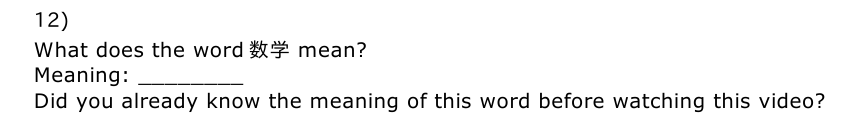
\includegraphics[width=\columnwidth]{vocab-quiz-1}
\caption{Vocabulary quiz question asking for the definition
of a word from the video, without providing the context it had appeared in.}
\label{fig:figure4}
\end{figure}

\begin{figure}[!h]
\centering
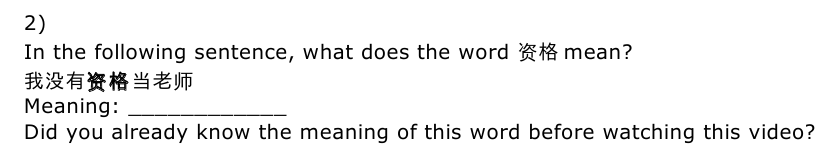
\includegraphics[width=\columnwidth]{vocab-quiz-2}
\caption{Vocabulary quiz question asking for the definition
of a word from the video, providing the context it had appeared in.}
\label{fig:figure5}
\end{figure}

For both types of questions, we additionally asked the participant to self-report whether they had known the meaning of the word before watching the video, so that we could determine whether it was a new word or one they had previously learned from some external source. This self-reporting mechanism is commonly used in vocabulary-learning evaluations for foreign-language learning \cite{wesche1996assessing}.

\subsubsection{Questionnaire}

After participants completed the vocabulary quiz, we asked them to write a summary of the clip they had
just seen, describing as many details as they could recall. Then, they completed
a questionnaire where they rated the following questions on a 7-point Likert scale:

\begin{itemize}[noitemsep]
\item How easy did you find it to learn new words while watching this video?
\item How well did you understand this video?
\item How enjoyable did you find the experience of watching this video with this tool?
\end{itemize}

Finally, we asked for free-form feedback about the user's impressions of the tool. %, and whether they would use the tool themselves.

\section{Results}

We found the following results from our study, which will be explained in
further detail in the following sections:

\begin{itemize}[noitemsep]
\item Users correctly defined over twice as many new words on the vocabulary quiz when using Smart Subtitles than with dual subtitles.
\item Viewing times did not differ significantly between the tools.
\item Viewers' self-assessed enjoyability did not differ significantly between the tools.
\item Viewers' self-assessed comprehension did not differ significantly between the tools.
\item Quality ratings of summaries viewers wrote did not differ significantly
between the tools.
\item Users made extensive use of both the word-level translations and the dialog-navigation features of Smart Subtitles, and described these as helpful.
\end{itemize}

\subsection{Vocabulary Learning}

Since the vocabulary quiz answers were done in free-response format, a third-party native Chinese speaker was asked to mark the learners' quiz answers as being either correct or incorrect. The grader was blind as to which condition or which learner the answer was coming from.

We measured the number of new words learned as the number of correctly defined words, excluding words that participants had marked as previously known. As shown in Figure~\ref{fig:figure6}, learners correctly answered more questions and correctly defined more new words when using Smart Subtitles. A t-test shows that there were significantly more questions correctly answered (t=3.49, df=7, p $<$ 0.05) and new words correctly defined (t=5, df=7, p $<$ 0.005) when using Smart Subtitles.
There was no significant difference in the number of words reported as known beforehand in each condition.

\begin{figure}[!h]
\centering
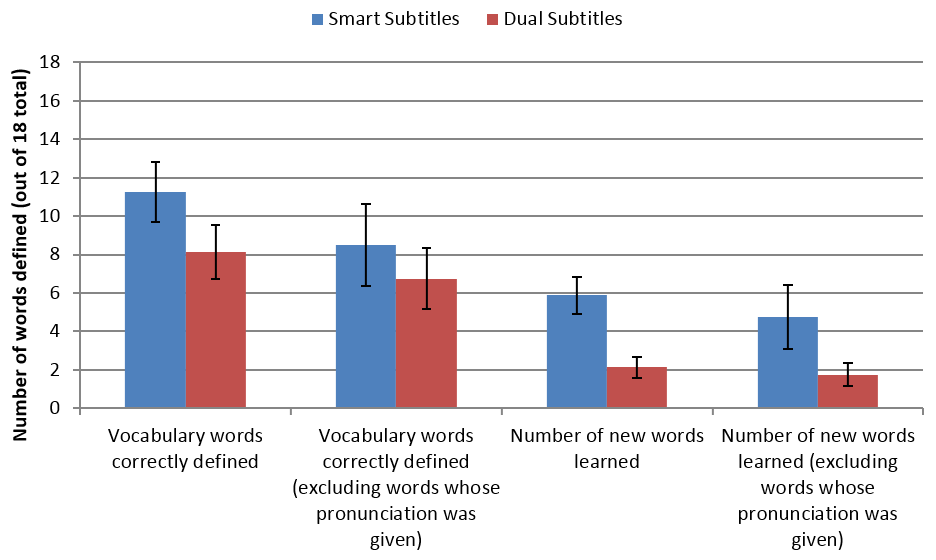
\includegraphics[width=\columnwidth]{vocab-quiz-results}
\caption{Vocabulary quiz results, with standard error bars.}
\label{fig:figure6}
\end{figure}

Although we did not evaluate pronunciation directly, Smart Subtitles' display of pinyin appeared to bring additional attention towards the vocabulary pronunciations. In our vocabulary quizzes, we gave the participants a synthesized pronunciation of the word, in the event that they did not recognize the Chinese characters. We opted to provide a synthesized pronunciation, as opposed to the pinyin directly, as they would not have been exposed to pinyin in the Dual Subtitles condition. This, predictably, allowed participants to correctly define a few additional words in both conditions. That said, there was a slightly increased level of gain in the Smart Subtitles condition when pronunciation was provided, with an additional 1.1 words correctly answered on average, than in the Dual Subtitles condition, with an additional .3 words correctly answered on average.

We attribute this to certain participants focusing more attention on the pronunciation, and less on the Chinese characters, in the Smart Subtitles condition. Indeed, one participant remarked during the vocab quiz for Dual Subtitles that she recognized some of the new words only visually and did not recall their pronunciations. We unfortunately did not ask participants to provide pronunciations for words, only definitions, so we cannot establish whether this held across participants.

\subsection{Viewing Times}

As shown in Figure~\ref{fig:figure7}, viewing times did not differ significantly between either of the two 5-minute clips, or between the tools. Viewing times were between 10-12 minutes for each clip, in either condition.
%Interestingly, the average viewing times with Smart Subtitles was actually %slightly less than with dual subtitles, which is likely due to the dialog-based %navigation features.
During the user study, we observed that users of Smart Subtitles would often review the vocabulary in the preceding few lines of the video clip by utilizing the interactive transcript, whereas users of Dual Subtitles would often over-seek backwards when reviewing, and would lose some time as they waited for the subtitle to appear.
Thus, the dialog-based navigation feature appears to have saved enough time in the Smart Subtitles condition to balance out any additional time spent using the interactive vocabulary learning features.

\begin{figure}[!h]
\centering
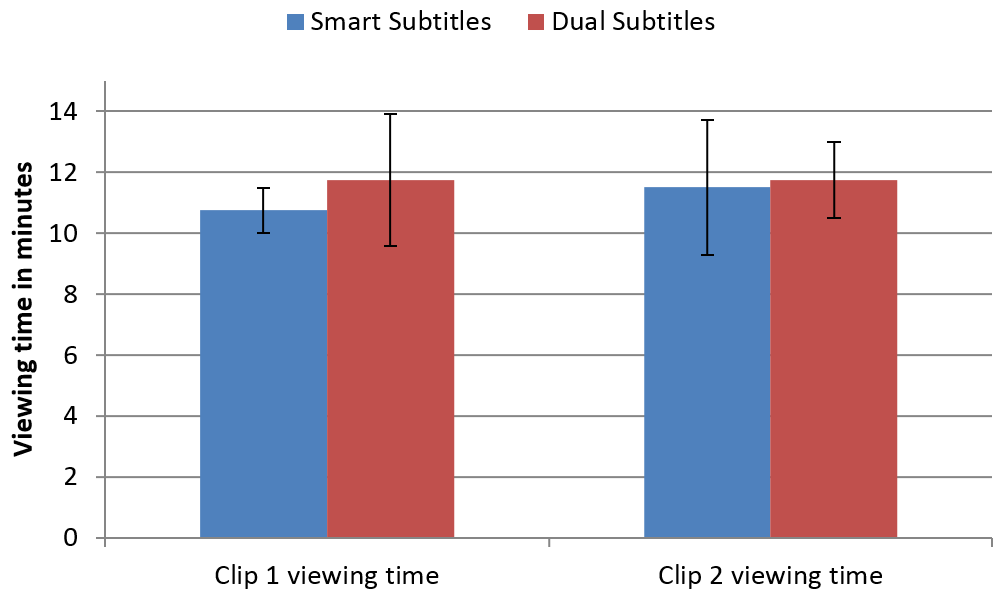
\includegraphics[width=\columnwidth]{viewing-times}
\caption{Viewing times, with standard error bars.}
\label{fig:figure7}
\end{figure}

\subsection{Self-Assessment Results}

As shown in Figure~\ref{fig:figure8}, responses indicated that learners considered it easier to learn new words with Smart Subtitles, (t=3.76, df=7, p $<$ 0.005), and rated their understanding of the videos as similar in both cases. The viewing experience with Smart Subtitles was rated to be slightly more enjoyable on average (t=1.90, df=7, p=0.08). Free-form feedback suggests that viewers' increased perceived ability to follow the original Chinese dialog contributed to the enjoyability of Smart Subtitles.

\begin{figure}[!h]
\centering
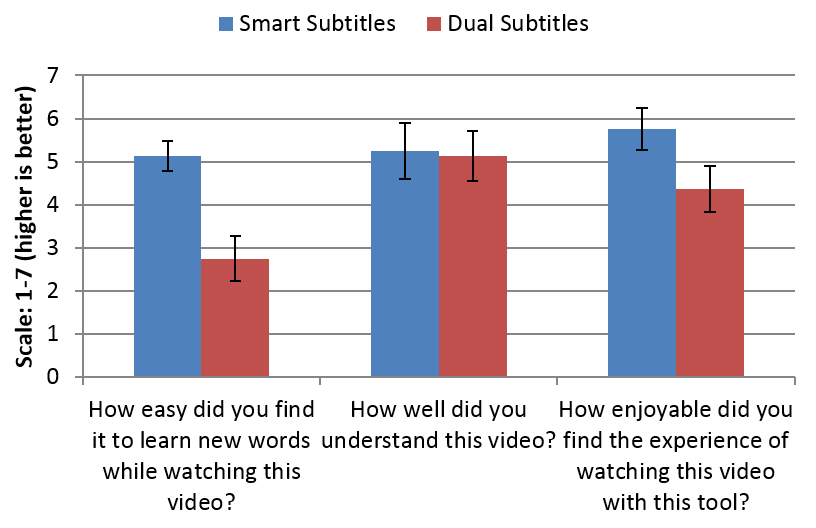
\includegraphics[width=\columnwidth]{self-assessment-results}
\caption{Self-assessment results, with standard error bars.}
\label{fig:figure8}
\end{figure}

\subsection{Summary Quality Ratings}

%After watching each video, partcipants wrote a summary describing the clip they had seen. An example is:

%\emph{It was about a failed teacher whose students don't take him seriously (they leave his class, want to beat him up), and then a president who is angry about his daughter doing poorly at math after hiring an expensive tutor.}

After watching each video, participants wrote a summary describing the clip they had seen.
To evaluate the quality of these summaries, we hired 5 Chinese-English bilingual raters to rate the summaries. The raters were hired from the oDesk contracting site, and were paid \$15 apiece. Raters were
first asked to view the clips, and write a summary in English to show that they had viewed and understood the clips.
Then, we presented them the summaries
written by students in random order. For each summary, we indicated which clip was being summarized, but the raters were blind as to which condition the student had viewed the clip under. Raters were asked to rate on a scale of 1 (worst) to 7 (best):

\begin{itemize}[noitemsep]
\item From reading the summary, how much does the student seem to understand this clip overall? %(7: completely seems to understand this part of the clip; 1: doesn't seem to understand it at all)
\item How many of the major points of this clip does this summary cover? %(7: covers enough major points in this part of the clip that the student seems to have understood the clip well; 1: the summary doesn't cover any of the major points)
\item How correct are the details in this summary of this clip? %(7: everything the student described in the summary was correct; 1: nothing the student described in the summary was correct).
\item How good a summary of this clip do you consider this to be overall? %(7: this is a good summary of this part of the clip; 1: this is a terrible summary of this part of the clip)
\end{itemize}

To ensure that the rater was actually reading the summaries and
was being consistent in their ratings,
we included one of the summaries twice in the list of summaries the
raters were asked to rate.
Two of our raters did not notice that these summaries were identical and
rated them differently, so we eliminated them for inconsistency.
Our conclusion about the summary quality not being significantly different between conditions would still have remained the same if we had included the ratings from these two raters.
Average rating results from the remaining three raters are shown in Figure~\ref{fig:figure9}.

\begin{figure}[!h]
\centering
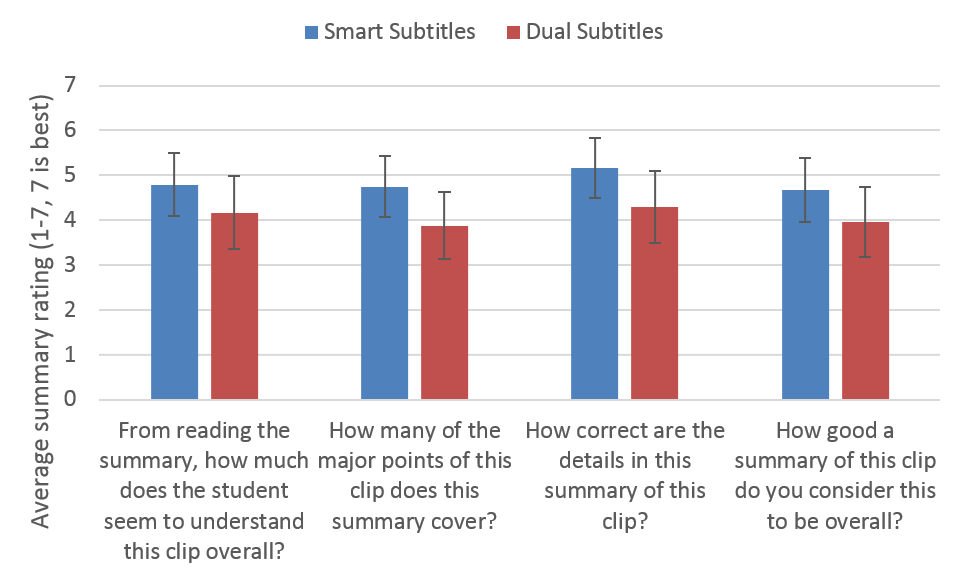
\includegraphics[width=\columnwidth]{summary-ratings}
\caption{Average ratings given by bilinguals on the quality of the summaries written by learners in each viewing condition.}
\label{fig:figure9}
\end{figure}

There was no significant difference in the quality of summaries written
by the learners between the Smart Subtitles and Dual Subtitles conditions,
according to any of the 4 quality metrics. The Krippendorff's alpha,
which measures agreement across raters \cite{krippendorff}, was 0.7.

%\subsection{Free-form Feedback}

%We asked users to provide feedback about the watching experience in general, and whether they were interested in using the tool again. Of our 8 users, all expressed interest in using Smart Subtitles again. The written feedback that participants wrote indicated that they found many of the interface features to be helpful, particularly the hover-over word definitions and video navigation features, though some found tone colorization to be distracting. %Here is, for example, an anecdote describing the navigation features:
	 	 	
%\emph{Yes! This was much better than the other tool. It was very useful being able to skip to specific words and sentences, preview the sentences coming up, look up definitions of specific words (with ranked meanings – one meaning often isn't enough), have pinyin, etc. I also really liked how the English translation isn't automatically there – I liked trying to guess the meaning based on what I know and looking up some vocab, and then checking it against the actual English translation. With normal subtitling, it's hard to avoid just looking at the English subtitles, even if I can understand it in the foreign language. This also helped when the summation of specific words did not necessarily add up to the actual meaning}

%The tone coloring feature in particular was not received as positively as the other features. The only comment on tone coloring was by one participant who described it as distracting. This would suggest that we may wish to simply remove this feature, or make the tones more salient using another means, such tone numbers, which are more visually apparent than tone marks.
	 	 	
%\emph{The tone coloring was interesting, but I actually found it a bit distracting. It seemed like I had a lot of colors going on when I didn't really need the tones color-coordinated. However, I think it's useful to have the tones communicated somehow.}

\subsection{Feature Usage during User Studies}

During our user studies, we instrumented the interface so that it would record actions such as dialog navigation, mousing over to reveal vocabulary definitions, and clicking to reveal translations for the current line of dialog.

Viewing strategies with Smart Subtitles varied across
participants, though all made some use of both
the word-level and dialog-line translation functionality.
Word-level translations were heavily used. On average,
users hovered over words in 75\% of the lines of dialog
($\sigma = 22\%$).
The words hovered over the longest tended to be less
common words, indicating that participants were using
the feature for defining unfamiliar words, as intended.
Participants tended to use dialog-line translations
sparingly. On average they clicked on the translate
button on only $28\%$ of the lines of dialog
($\sigma = 15\%$).
Combined with our observation that there was no decline in
comprehension levels with Smart Subtitles, this suggests
that word-level translations are often sufficient for
intermediate-level learners to understand dialogs.

\subsection{Study Limitations}

Although our pilot study shows promising results,
further studies are needed to assess
this system's overall effectiveness for long-term language learning.
In particular, because vocabulary quizzes were administered immediately
after viewing the 5-minute clips,
this study tests only short-term vocabulary retention.
Additionally, as we asked on learners to self-report whether they had previously known words,
instead of using a pre-test,
this could have led to measurement errors.
Our participants were also limited to intermediate-level learners who had taken a year
of courses,
so further studies are needed to determine whether this video-viewing approach can be used by
novices with no prior exposure to the language, or whether novices require additional scaffolding.

\section{Conclusion and Future Work}

We have presented Smart Subtitles, an interactive
video viewer which features vocabulary
definitions on hover and dialog-based video navigation
to help language learners learn vocabulary while watching videos.
They can be automatically generated from
common sources of videos and subtitles, such as DVDs.

Our pilot study found that intermediate-level learners correctly defined more
new words in a vocabulary quiz administered after viewing, when viewing with Smart Subtitles
compared to dual Chinese-
English subtitles. They spent the same amount of time viewing, and rated their comprehension and
enjoyment of the video as similarly high.
Independent ratings of summaries written by participants
further confirm that comprehension levels when using Smart Subtitles
match those when using dual subtitles.

Although OCR and machine translation
allow Smart Subtitles to be automatically generated for a large body of content,
we will need a means to correct errors from these systems,
or generate transcripts from scratch if no transcript sources are available.
We can address this by maintaining an online database of transcripts
that have been corrected by users in a wiki-like fashion, and using video fingerprinting % cite?
to automatically fetch the appropriate transcript when viewing videos.

Much work can still be done in the area of incorporating multimedia into learning. Our current Smart Subtitles system focuses on written vocabulary learning while watching dramas and movies.
However, we believe that augmenting video can also benefit other aspects of language learning. For example, we could
incorporate visualizations to help teach grammar and sentence patterns,
and speech synthesis to help teach pronunciation. We could also 
pursue further gains in vocabulary learning and comprehension,
by dynamically altering the video playback rate, or by adding
quizzes into the video to ensure that the user is continuing to pay attention.

Other multimedia forms can likewise benefit from interfaces geared
towards language learning, though each form comes with its own
unique challenges. For example, the current Smart Subtitles system can
easily be used with existing music videos and song lyrics.
However, the system would be even more practical for music if
we could remove the need for an interactive display, and simply
allow the user to learn while listening to the music.
Multimedia that is naturally interactive, such as Karaoke,
likewise presents interesting opportunities for
making boring tasks, such as practicing pronunciation, more interesting
to learners.

We hope our work leads to a future where people can learn foreign languages more enjoyably by being immersed in foreign multimedia, while reducing the effort that needs to be dedicated towards making the material education-friendly. %or even fully translating it.

\section{Acknowledgements}

This work is supported in part by Quanta Computer as 
part of the T-Party project. Thanks to Chen-Hsiang Yu and Carrie Cai for advice
on study design.

\balance

% REFERENCES FORMAT
% References must be the same font size as other body text.

\bibliographystyle{acm-sigchi}

\bibliography{smartsubs-paper}

\end{document}
